\section{Contamination from Lensing}

We now consider gravitational lensing of the 21-cm signal by the large scale structure, as a source of noise in searches for magnetic fields using the method proposed in this work. We first compute the transverse shear power spectrum and then evaluate the bias it produces for the magnetic-field estimator.

In order to follow standard lensing notation, we no longer label cartesian coordinate axes with $x$, $y$, and $z$, but rather with numbers, using the convention where directions labeled as $1$ and $2$ lie in the plane of the sky, while $3$ lies along the line of sight. Specifically, we use angular coordinates $(\theta_1, \theta_2)$ to denote direction in the sky ${\bf{\widehat n}}$, and $\theta_3$ to denote a comoving interval $r_z/\chi(z)$ along the line of sight, located at redshift $z$, and corresponding to $\Delta z$. As before, we denote variables in Fourier space with tilde, and use $\vec{\ell}\equiv(\ell_1,\ell_2)$ for a conjugate variable of ${\bf{\widehat n}}$. 
 
We start by adopting the formalism for two-dimensional weak lensing \cite{Weinberg201387} to the case where lensed sources are spread out in three dimensions. In the presence of lensing, coordinate $\theta_i^S$, where $i\in\{1,2,3\}$, maps onto the observed coordinate $\theta_i$ as follows \begin{equation}
\theta_i^S=\theta_i+\frac{\partial\psi}{\partial\theta_i},\ i=1,2,3,
\label{eq:lensingmapping}
\end{equation}
where $\psi$ is the lensing potential. The full Jacobian of this coordinate transformation is
\begin{equation}
\frac{\partial\theta_i^S}{\partial\theta_j}=\delta_{ij}+\frac{\partial^2\psi}{\partial\theta_i\partial\theta_j}=(1+\kappa)I_{ij}+\gamma_{ij},\ \ \ i,j=1,2,3,
\label{eq:lensingtsf}
\end{equation}
where $I_{ij}$ represents the unity matrix. In the second step in the above equation we decomposed the symmetric $3\times 3$ matrix $\partial^2\psi/\partial\theta_i\partial\theta_j$ into a sum of a diagonal and a symmetric traceless matrix $\bm{\gamma}$, representing magnification and shear, respectively. There are five independent shear components.
%The $\tilde{\gamma}_{13},\tilde{\gamma}_{23}$ components are the transverse shear components that we care about. Let's calculate the power spectrum of $\gamma_{13}$ first.

We now switch to Fourier space, where the two-dimensional Fourier transform of the lensing potential reads
\begin{equation}
\widetilde{\psi}(\vec{\ell},z)\equiv\int\psi({\bf\widehat{n}},z)e^{-i\vec{\ell}\cdot{\bf{\widehat n}}}\ d\theta_1 d\theta_2.
\label{eq:potentialFourier}
\end{equation}
The relation between $\psi$ and the Newtonian potential $\Phi$ in a flat universe is
\begin{equation}
\psi({\bf{\widehat n}},z)=
-2\int_0^{\chi(z)}d\chi_1\left[\frac{1}{\chi_1}-\frac{1}{\chi}\right]\Phi({\bf{\widehat n}},\chi_1),
\label{eq:lensingpotential}
\end{equation}
where $\chi_1$ is an integration variable.
Combining Eqs.~(\ref{eq:potentialFourier}) and (\ref{eq:lensingpotential}), we get 
\begin{equation}
\frac{\partial\widetilde{\psi}(\vec{\ell},z)}{\partial\theta_3}=-\frac{2}{\chi(z)}\int_0^{\chi(z)} d\chi_1\widetilde{\Phi}(\vec{\ell},\chi_1).
\label{eq:dpsi_dtheta3}
\end{equation}
From Eqs.~(\ref{eq:dpsi_dtheta3}) and (\ref{eq:lensingtsf}), it follows 
\begin{align}
&\langle\widetilde{\gamma}_{13}^*(\vec{\ell},z)\widetilde{\gamma}_{13}(\vec{\ell}',z')\rangle=\left\langle \ell_1\ell_1'\frac{\widetilde{\psi}^*(\vec{\ell},z)}{\partial\theta_3}\frac{\widetilde{\psi}(\vec{\ell}',z')}{\partial\theta_3}\right\rangle\nonumber\\
&=\frac{4\ell_1\ell_1'}{\chi(z)\chi(z')}\int_0^{\chi(z)}d\chi_1\int_0^{\chi(z')}d\chi_1'\langle\widetilde{\Phi}^*(\vec{\ell},\chi_1)\widetilde{\Phi}(\vec{\ell}',\chi_1')\rangle.
\end{align}

We now define the three-dimensional Fourier transform of the Newtonian potential $\widetilde{\widetilde\Phi}$ through
\begin{equation}
\widetilde{\Phi}(\vec{\ell},\chi)\equiv\int\widetilde{\widetilde{\Phi}}(\vec{\ell},\ell_3)e^{i\ell_3\chi}\frac{d\ell_3}{2\pi},
\end{equation}
where $\ell_3$ is an integration variabe. Using this definition, we get
\begin{align}
\langle\widetilde{\Phi}^*(\vec{\ell},\chi)\widetilde{\Phi}(\vec{\ell}',\chi')\rangle=\int\int&\frac{d\ell_3}{2\pi}\frac{d\ell_3'}{2\pi}\langle\widetilde{\widetilde{\Phi}}^*(\vec{\ell},\ell_3)\widetilde{\widetilde{\Phi}}(\vec{\ell}',\ell_3')\rangle\nonumber\\
&\times e^{i(\ell_3'\chi'-\ell_3\chi)}. \label{eq:doubletilde}
\end{align}
Assuming different modes are uncorrelated, we get
\begin{equation}
\bga
\langle\widetilde{\widetilde{\Phi}}^*(\vec{\ell},\ell_3)\widetilde{\widetilde{\Phi}}(\vec{\ell}',\ell_3')\rangle\\
=(2\pi)^3\delta(\ell_3-\ell_3')\delta^2(\vec{\ell}-\vec{\ell}')P_{\Phi}(\sqrt{\ell_3^2+\ell^2}).
\ega
\label{eq:expectation_tildetildephi}
\end{equation}
where
\begin{equation}
\bga
P_{\Phi}(\ell)=\frac{P_{\Phi}(k=\ell/\chi(z))}{\chi(z)^2}\\
=\left[\frac{3}{2}\Omega_mH_0^2(1+z)\right]^2\frac{P_{\delta}(k,z)}{k^4\chi(z)^2},
\ega
\end{equation}
is the angular power spectrum.
Substituting Eq.~(\ref{eq:expectation_tildetildephi}) into (\ref{eq:doubletilde}) and applying Limber approximation $\ell_3\ll\ell$, we obtain
\begin{equation}
\langle\widetilde{\Phi}^*(\vec{\ell},\chi)\widetilde{\Phi}(\vec{\ell}',\chi')\rangle=(2\pi)^2\delta^2(\vec{\ell}-\vec{\ell}')P_{\Phi}(\vert\vec{\ell}\vert)\delta(\chi'-\chi),
\end{equation}
Thus, for $z\leq z'$,
\beq
\bga
\langle\widetilde{\gamma}_{13}^*(\vec{\ell},z)\widetilde{\gamma}_{13}(\vec{\ell}',z')\rangle\\
=\frac{4}{\chi(z)\chi(z')}\ell_1\ell_1'(2\pi)^2\delta^2(\vec{\ell}-\vec{\ell}')\int_0^{\chi(z)}d\chi_1P_{\Phi}(\ell).
\ega
\label{eq:exp_gamma13}
\eeq

We are interested in calculating the power spectrum $P_{13}(\vec{\ell},z,z')$ of $\gamma_{13}$ components, defined as
\begin{equation}
\bga
\langle\widetilde{\gamma}_{13}^*(\vec{\ell},z)\widetilde{\gamma}_{13}(\vec{\ell}',z')\rangle\equiv(2\pi)^2P_{13}(\vec{\ell},z,z')\delta^2(\vec{\ell}-\vec{\ell}').
\ega
\end{equation}
From Eq.~(\ref{eq:exp_gamma13}) we can express
\begin{equation}
P_{13}(\vec{\ell},z,z')=\frac{4\ell_1^2}{\chi(z)\chi(z')}\int_0^{\chi(z)}d\chi_1P_{\Phi}(\ell),
\end{equation}
where as before, $\chi_1$ is an integration variable.
Similar result holds for the power spectrum $P_{23}$ of $\gamma_{23}$ component. Finally, the transverse power spectrum $P_t$ can be expressed as 
\beq
\bga
P_t(\ell,z,z')\equiv P_{13}+P_{23}\\
=\frac{4\ell^2}{\chi(z)\chi(z')}\int_0^{\chi(z)}d\chi_1P_{\Phi}(\ell).
\ega
\eeq
If $z=z'$, the above expression simplifies to
\begin{equation}
P_t(\ell,z)=\frac{4\ell^2}{\chi(z)^2}\int_0^{\chi(z)}d\chi_1P_{\Phi}(\ell).
\end{equation}
In Fig.~\ref{fig:Pt}, we show the transverse power spectra for a range of $z$, for standard cosmology.
\begin{figure}
\centering
\includegraphics[scale=0.45]{lensing_transverse.pdf}
\caption{The transverse power spectra for sources at redshifts $z=10$, $20$ and $30$, computed for standard cosmology.}
\label{fig:Pt}
\end{figure}

Now that we have computed the transverse power spectrum $P_t$, we move on to evaluating the contamination it produces for the measurement of the magnetic field. To do that, we start by considering a configuration where the magnetic field is along the direction labeled as ``2'', ${\bf{\widehat k}}=(\sin\varphi,0,\cos\varphi)$, and the line of sight is along the direction ``3'' $\ {\bf{\widehat n}}=(0,0,1)$ in the three-dimensional Cartesian reference frame we adopted in this Appendix; $\varphi$ is the angle between the direction ``3'' and ${\bf{\widehat k}}$. Due to lensing, the latter two unit vectors are distorted into, respectively,
\begin{align}
{\bf{\widehat k}}'&=\left(\begin{array}{c}
(1+\kappa+\gamma_{11})\sin\varphi+\gamma_{13}\cos\varphi\\
\gamma_{12}\sin\varphi+\gamma_{23}\cos\varphi\\
\gamma_{13}\sin\varphi+(1+\kappa+\gamma_{33})\cos\varphi
\end{array}\right),\nonumber\\
{\bf{\widehat n}}'&=\left(\begin{array}{c}
\gamma_{13}\\
\gamma_{23}\\
1+\kappa+\gamma_{33}
\end{array}\right)
\label{eq:distorted_kn}
\end{align}





.......

\subsection{Lensing Bias}
Ref.~\cite{Venumadhav:2014tqa} has found the expression of the brightness temperature fluctuation $\delta T_b$ as a function of the magnitude of magnetic fields, i.e.~Eq.~(\ref{}). To make the derivation concise, we define several quantities as below.
\begin{align}
\bar{x}_{\rm B}&\equiv\frac{x_{\rm B}}{B} = \frac{g_{\rm e} \mu_{\rm B} T_*}{2 \hbar A T_\gamma},\\
A&\equiv\left( 1 - \frac{T_\gamma}{T_{\rm s}} \right) x_{1{\rm s}} \left( \frac{1+z}{10} \right)^{1/2},\\
C&\equiv0.128 \ {\rm mK} \left( \frac{T_\gamma}{T_{\rm s}} \right) x_{1{\rm s}} \left( \frac{1+z}{10} \right)^{1/2},\\
\mu&\equiv\frac{C}{10}\frac{x_B}{(1+x_{\alpha,(2)}+x_{c,(2)})^2},\\
\lambda&\equiv 13.2-C-\frac{C}{20}\frac{1}{1+x_{\alpha,(2)}+x_{c,(2)}},\\
q&\equiv 39.6-3C-\frac{C}{60}\frac{1}{1+x_{\alpha,(2)}+x_{c,(2)}}.
\end{align}


The power spectrum of the brightness temperature is related to the matter power spectrum $P_\delta(k)$ by
\begin{equation}
P_{T_b}(\bm k)=\left\vert\frac{\partial\delta T_b}{\partial\delta}\right\vert^2 P_\delta(k).
\end{equation}
The transfer function $\partial\delta T_b/\partial\delta$ is given by taking derivative of Eq.~(\ref{}), i.e.~\begin{eqnarray}
\frac{\partial\delta T_b}{\partial\delta}&&=A\left[(26.4-2C)\left(1 + (\hat{\bm k} \cdot \hat{\bm n})^2\right)\right. \nonumber\\
&&\left.-\frac{C}{15}\sum_m \frac{4\pi}{5}\frac{Y_{2m}(\hat{\bm k})[Y_{2m}(\hat{\bm n})]^*}{1+x_{\alpha,(2)}+x_{c,(2)}-imx_B}\right],
\label{eq:bttsf}
\end{eqnarray}

By expanding Eqn.(\ref{eq:bttsf}) for small magnetic field $B$ (small $x_B$), we will obtain a precession correction on the original $P_{T_b}$ profile. The tangent of the precession angle $\theta_{pr}$ is proportional to the magnitude of the magnetic field applied.

To see that, let's first define our coordinate system as shown in Fig.\ref{fig:coordinate}. The unit vectors then will be $\hat{k}=(\pi/2,\varphi)$ and ${\bf{\widehat n}}=(\pi/2,0)$, where the first coordinate represents the angle between the Direction \#2 and the vector. The expansion becomes
\begin{equation}
\frac{\partial\delta T_b}{\partial\delta}=A(q+\lambda\cos 2\varphi+\mu\sin 2\varphi).
\label{eq:Tbtsf_simplified}
\end{equation}
\begin{figure}
\centering
\includegraphics[scale=0.3]{coordinate.pdf}
\caption{The coordinate system}
\label{fig:coordinate}
\end{figure}

Due to the $\sin 2\varphi$ term contributed by the small magnetic field, the original profile gets a small precession angle $\theta_{pr}$
\begin{equation}
\theta_{pr}\simeq\tan\theta_{pr}=-\frac{\mu}{\lambda},
\end{equation}

Thus, if we measure the precession angle $\theta_{pr}$ in the power spectra of $T_b$, we can determine the magnitude of the magnetic field.

Next we will show that the transverse components of the weak lensing can also produce a similar precession angle.

In the 3D Cartesian coordinate, the unit vectors are written as
\begin{equation}
\hat{k}=(\sin\varphi,0,\cos\varphi),\ {\bf{\widehat n}}=(0,0,1),
\end{equation}
and they are distorted into
\begin{align}
\hat{k}'&=\left(\begin{array}{c}
(1+\kappa+\gamma_{11})\sin\varphi+\gamma_{13}\cos\varphi\\
\gamma_{12}\sin\varphi+\gamma_{23}\cos\varphi\\
\gamma_{13}\sin\varphi+(1+\kappa+\gamma_{33})\cos\varphi
\end{array}\right),\nonumber\\
{\bf{\widehat n}}'&=(\gamma_{13},\gamma_{23},1+\kappa+\gamma_{33}).
\end{align}
Since the shearing components are all very small, by taking the first order, we obtain the shear only change $\varphi$ by
\begin{equation}
\Delta\varphi\simeq\sin\Delta\varphi\simeq-2\gamma_{13}.
\end{equation}
Thus, if there is no magnetic field ($x_B=0$), due to the weak lensing, the transfer function (\ref{eq:Tbtsf_simplified}) will become
\begin{equation}
\frac{\partial\delta T_b}{\partial\delta}=A[q+\lambda(\cos 2\varphi+4\gamma_{13}\sin 2\varphi)].
\label{eq:Tbtsf_shear}
\end{equation}
Since the weak lensing also spurs the $k$ in $P_\delta(k)$, we need to find the relation between $P_\delta(k')$ and $P_\delta(k)$. To the first order, we can find
\begin{equation}
k'=k(1+\kappa+\gamma_{11}\sin^2\varphi+\gamma_{33}\cos^2\varphi+2\gamma_{13}\sin\varphi\cos\varphi).
\end{equation}
Since $P_\delta(k)\propto k^{n_{\rm eff}}$, we have
\begin{align}
P_{T_b}(\vec{k}')=&\left\vert\frac{\partial\delta T_b}{\partial\delta}[1+\kappa+\gamma_{11}\sin^2\varphi+\gamma_{33}\cos^2\varphi\right.\nonumber\\
&\left.+2\gamma_{13}\sin\varphi\cos\varphi]^{n_{\rm eff}/2}]\right\vert^2P_\delta(k),
\end{align}
where $n_{\rm eff}$ is the effective spectral index. We can see all the quadropole features in the power spectra of $T_b$ come from the modified transfer function.

After expanding, keeping the first-order terms and neglecting small octupole terms, we can obtain the modified transfer function, and find the precession angle again, given by the negative ratio of the two coefficients of the quadrupole terms,
\begin{equation}
\theta_{pr}'\simeq-\left(4+\frac{n_{\rm eff}}{2}\frac{q}{\lambda}\right)\gamma_{13}.
\end{equation}
This precession angle is made by the transverse weak lensing component instead of the magnetic field, but the effect it makes looks like there is a (fake) magnetic field such that
\begin{equation}
\frac{\mu}{\lambda}=\left(4+\frac{n_{\rm eff}}{2}\frac{q}{\lambda}\right)\gamma_{13},
\end{equation}
where we can solve for the (fake) comoving magnetic field
\begin{align}
B_{\rm lensing,13}&=\frac{10(1+x_{\alpha,(2)}+x_{c,(2)})^2(4\lambda+\frac{n_{\rm eff}}{2}q)}{C\bar{x}_{\rm B}(1+z)^2}\gamma_{13}\nonumber\\
&\equiv\alpha\gamma_{13}.
\end{align}
Finally, we find the power spectrum of the comoving lensing magnetic field
\begin{equation}
P_B^{\rm lensing,13}(\ell)=\left\vert\frac{\partial B_{\rm lensing,13}}{\partial\gamma_{13}}\right\vert^2 P_{\gamma_{13}}(\ell)=\alpha^2 P_{\gamma_{13}}(\ell).
\end{equation}
Note that this power spectrum is only the contribution from $\gamma_{13}$ component because we assume $\hat{k}$ to sit on the "1-3" plane. For any position on the sky, one has the choice to rotate his coordinate system to maximize or minimize $P_{13}$. However, randomly, the total power spectrum of comoving lensing magnetic field picks up an average value, i.e.~the half maximum,
\begin{equation}
P_B^{\rm lensing}(\ell)=\frac{\alpha^2}{2} P_t(\ell),
\end{equation}
\begin{equation}
\Delta_{B}^{\rm lensing}(\ell)=\sqrt{\frac{l(l+1)}{2\pi}P_B^{\rm lensing}(\ell)}
\end{equation}

For a survey with $\Omega_{\rm survey}=1{\rm sr}$, the scale of interest is about $l=6$. The scale of matter fluctuations relavant to the observed signals is determined by the resolution of the inferometers as
\begin{equation}
k\sim \frac{2\pi L}{\lambda_0(1+z)D}\sim 1,
\end{equation}
corresponding to $n_{\rm eff}\sim -2.274$.

\begin{figure}[h]
\centering
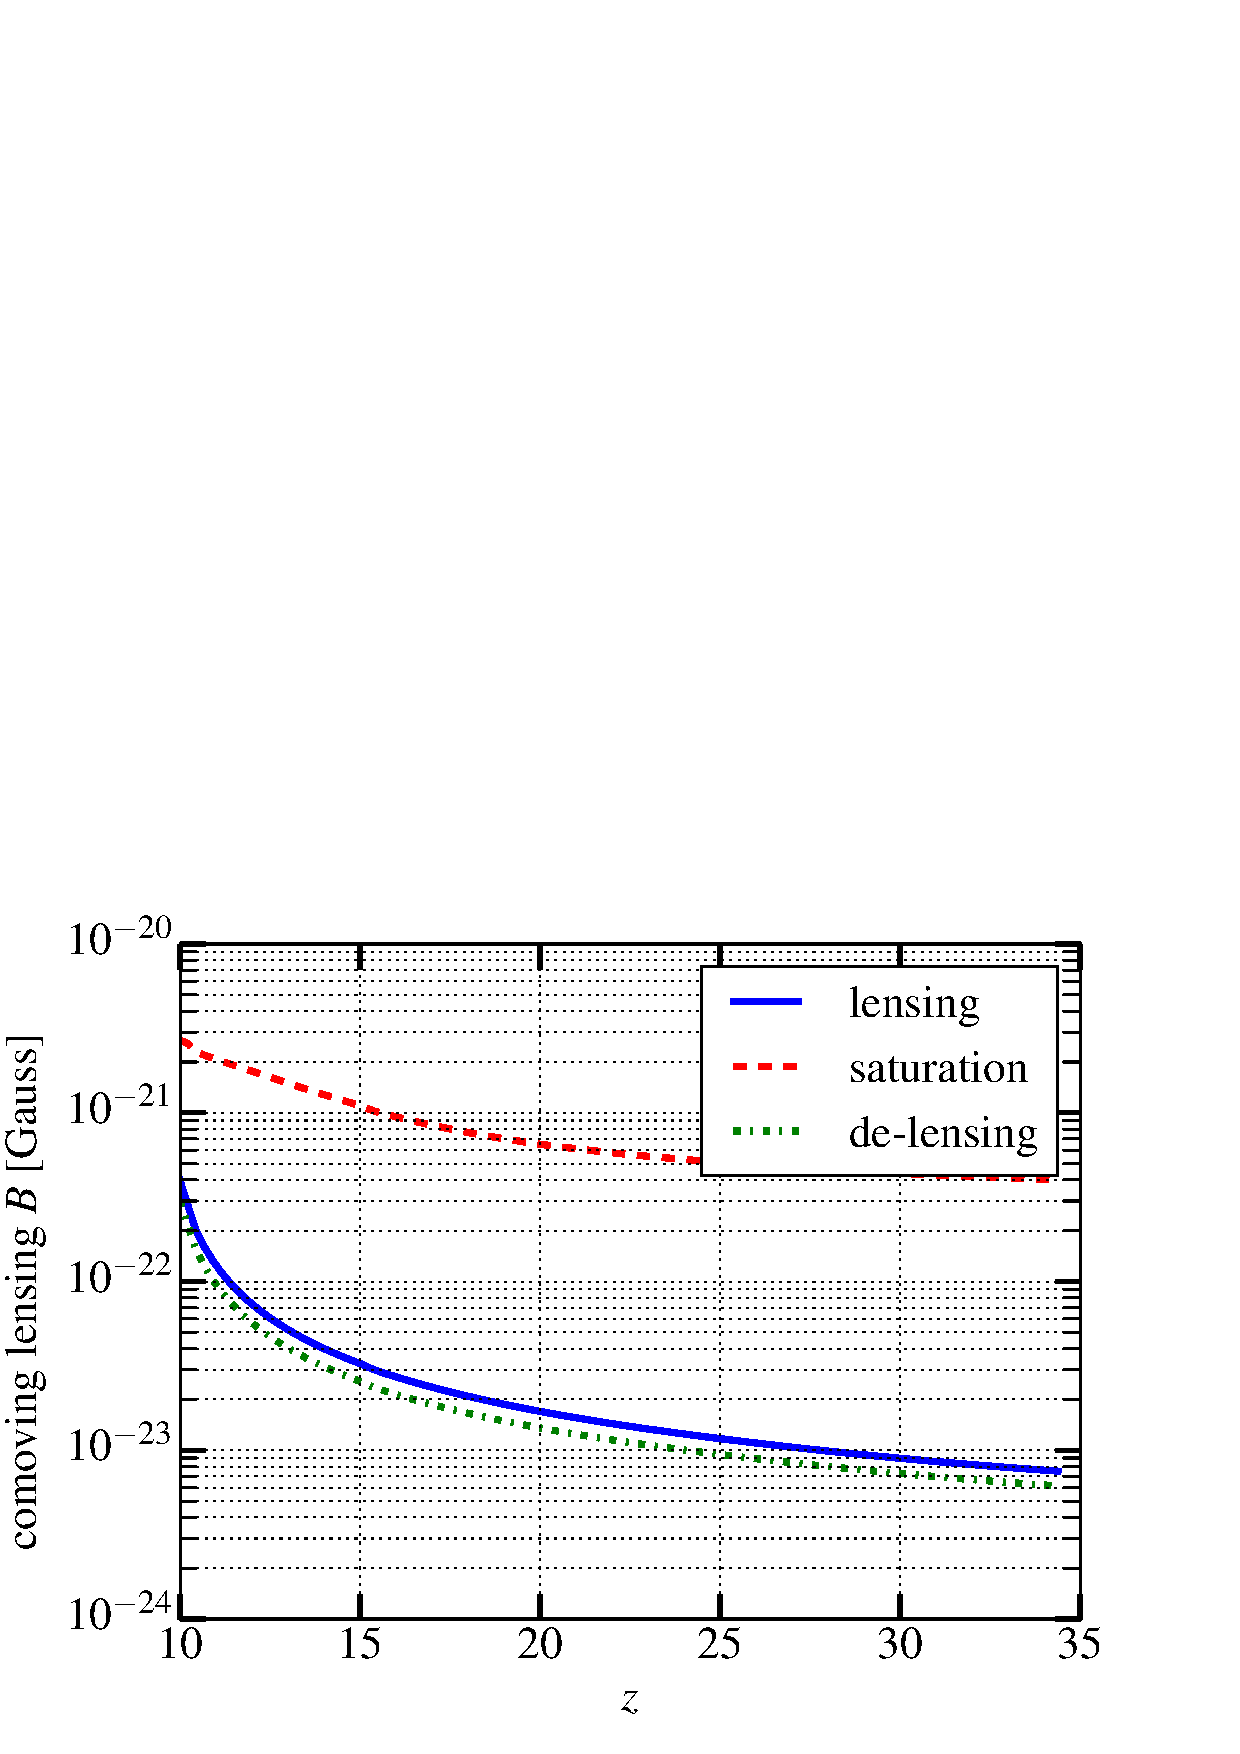
\includegraphics[scale=0.4]{delensingB.pdf}
\caption{The $1\sigma$ comoving lensing magnetic field before and after de-lensing, as produced by the transverse shearing effect of weak lensing, compared to the saturation limit of our method.}
\label{fig:ps_B}
\end{figure}
